\documentclass[letterpaper,11pt]{article}
\usepackage{fixltx2e} % LaTeX patches, \textsubscript
\usepackage{cmap} % fix search and cut-and-paste in Acrobat
\usepackage{ifthen}
\usepackage[T1]{fontenc}
\usepackage[utf8]{inputenc}
\usepackage{longtable,ltcaption,array}
\usepackage{fullpage}
\usepackage{multicol}
\usepackage{graphicx}
\usepackage{wrapfig}
\newlength{\DUtablewidth} % internal use in tables

%%% Custom LaTeX preamble
% PDF Standard Fonts
\usepackage{mathptmx} % Times
\usepackage[scaled=.90]{helvet}
\usepackage{courier}

%%% User specified packages and stylesheets

%%% Fallback definitions for Docutils-specific commands

\usepackage[colorlinks=true,linkcolor=blue,urlcolor=blue]{hyperref}
\urlstyle{same} % normal text font (alternatives: tt, rm, sf)

%\title{
%\author{}

\begin{document}

\begin{center}
	\LARGE
	\color{red}
	Interactive Parallel Post-Processing of \\
	Advanced Simulation Code Output
\end{center}

\vspace{0.5in}

\setlength{\parindent}{0pt}
\large
Laboratory Directed Research and Development \\
Lawrence Livermore National Laboratory \\
Lab Wide - New proposal

\normalsize
\begin{multicols}{2}
\textbf{Principle Investigator:}
\columnbreak

Matthew R. Terry \\
Physicist, Fusion Energy Program \\
Heavy Ion Fusion Virtual National Laboratory \\
Physics and Life Sciences Division

\end{multicols}


\textbf{Co-Investigators:}
\begin{multicols}{2}
	David Grote \\
	Fusion Energy Program \\
	Physics and Life Sciences Division\\
	\columnbreak
			
	Anthony Scopatz \\
	The FLASH Center for Computational Science \\
	Department of Astrophysics \\
	The University of Chicago \\
\end{multicols}

%\textbf{Collaborators:}
%\begin{multicols}{2}
%    Joe Koning \\
%    HYDRA \\
%    Engineering Division \\

%    Cyrus Harrison \\
%    VisIt, Somewhere \\
%    Compuational Division(?) \\
%    \columnbreak

%    Dag Sverre Seljebotn \\
%    University of Oslo \\

%    Travis Oliphant (?) \\
%    Continuum Analytics \\
%\end{multicols}


\setlength{\parindent}{15pt}
%___________________________________________________________________________

\section*{Executive Summary }
We propose the research and development of an interactive computing platform capable of 
processing massively-parallel memory distributed arrays.  The advent of parallel 
computing devices has led to dramatic improvements in the scope and fidelity of 
computational science.  However, these advances have largely left interactive computing 
behind.  There are specialized tools for visualizing large datasets (such as 
VisIt\cite{VisIt}), but these do not solve the problem of needing to directly manipulate 
large datasets \emph{interactively}.  The inability to interactively manipulate large 
datasets restricts both the scope and the pace of research, particularly at LLNL where 
large scale simulation is common.  Therefore, we propose the development of a platform 
with the following capabilities:

\begin{enumerate}
	\item A distributed n-dimensional array, capable of loading too-large-for-serial meshes 
          and having a high-level interface which automatically handles how 
          the array is physically distributed.

	\item A powerful, modern interactive shell with name completion, syntax highlighting, 
		descriptive error messages, etc.  It will familiar to users of Mathematica, 
		MatLab, Yorick, Basis, etc.

	\item Data sharing between the interpreted platform and high quality visualization tool VisIt.
\end{enumerate}

The critical areas of research are identifying how general the array distribution can be 
while maintaining acceptable performance and identifying how many details of the array 
distribution to require the user to specify.  The initial application of this platform 
will target processing of output from LLNL's HYDRA\cite{Marinak2001} radiation-hydrodynamics 
code, but all of the infrastructure will be directly useful for of LLNL's structured mesh 
(HYDRA, LASNEX\cite{Zimmerman1977}), automatic mesh refinement
(Warp\cite{Grote2005}, FLASH\cite{flash}, ALE-AMR\cite{Koniges2010}, ARES\cite{needed}),
and unstructured mesh codes (KULL\cite{Rathkopf2000}).  The platform builds on the vibrant
Python scientific computing ecosystem, particularly the NumPy\cite{Oliphant2006}, 
SciPy\cite{numpyscipy}, IPython\cite{ipython} and VisIt projects.

%___________________________________________________________________________

\section*{Technical Description}

After 50 years of concerted effort, LLNL stands on the verge of demonstrating inertial 
confinement fusion (ICF) ignition and energy gain on the National Ignition Facility\@.
ICF involves compressing a spherical shell cryogenic Deuterium and Tritium ice (Hydrogen isotopes) by a factor of approximately 35.  In this processes, the shell implodes with a 
velocity of 350 km/s, achieves densities greater than
xx g/cm${}^3$ and temperatures in
excess of 100,000,000 K.  The implosion is driven by high intensity laser beams heating 
the inner surface of a Gold cylinder called a ``hohlraum.''  The hohlraum radiates x-rays 
which impinge on the shell and drive the implosion.  Figure~\ref{hohlraum} give a schematic.  Simulating such experiments requires accurate modeling of
hydrodynamics, (photon) sophisticated radiation transport, thermal conduction, equations 
of state spanning from cryogenic to thermonuclear, laser propagation, fusion burn, and more.
In this, HYDRA occupies a central role in designing NIF experiments and in interpreting the experimental data gathered.  HYDRA is massively parallel, code developed in AX Division
capable of describing all the mentioned physical processes in 3 dimensions.

\begin{wrapfigure}{r}{0.45\textwidth}
	\vspace{-25pt}
	\begin{center}
		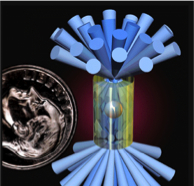
\includegraphics[width=0.40\textwidth]{hohlraum.jpg}
	\end{center}
	\caption{Schematic of ICF hohlraum (yellow), laser beams (blue) and capsule inside the hohlraum.}
	\label{hohlraum}
\end{wrapfigure}

% TODO
To motivate this proposal, consider the quantity of data generated
by a large 3D HYDRA simulation.  A large simulation can:
have
	xx grid points,
run on 
	xx processors,
consume 
	xx TB of RAM and
produce 
	xx TB of binary data.  When examining the output of such a simulation, loading the
just the computational mesh, at a single snapshot in time consumes
	xx GB RAM\@.  For a sense of scale, Inca, which has the largest per-node RAM allocation 
at Livermore Computing, has 48 GB\@.  Clearly, the output of our simulation codes has grown
beyond our ability to load and manipulate on a single computer node.

The bedrock data structure in scientific computing is the n-dimensional array (nd-array).  
It is a memory-contiguous sequence of data of uniform type.  It has the convenient property 
of resembling both a linear algebra vector/matrix/tensor as well as a being a data structure
with good performance.  Due to its ubiquity, there are many high level programming 
languages that have language-level support (MatLab\cite{matlab}, Yorick\cite{Munro1995}), 
or widely used libraries (Python\cite{CPython} via NumPy\cite{Oliphant2006}) for 
manipulating nd-arrays.  The long-term popularity of Fortran for scientific computing is 
due in part to its excellent support for nd-arrays.  These languages are useful across 
many scientific domains because they leverage the mutual abstraction of the nd-array.

Programs written for distributed memory computers still leverage the nd-array, but scatter 
the array memory across many machines (``distributed array'').  This allows for arrays 
with memory requirements larger than the capacity of a single machine \emph{and} divides 
the computational work among many processors.  While the distributed array data structure 
is very common, there is neither a standard implementation nor direct language support.  
The lack of a standard abstraction forces each project to write their own data structure 
which are often incompatible with other implementations.  This significantly inhibits code
and tool reuse and slows the evolution of scientific software.

In particular, the lack of a standard distributed array means that very high-level 
languages have not taken such an object and provided a simplified, idiomatic interface.
Thus, processing large datasets is largely confined to special purpose software which is 
not available to all computational scientists.

We propose the development of a distributed array package for Python that follows NumPy's 
tradition of interoperability and adaptability.  Like NumPy's \texttt{ndarray}, this 
distributed array will be able wrap pre-existing distributed data structures and provide 
an alternate interface without copying or substantially modifying the original program.  
The distributed array will work with HDF5\cite{HDF5} and SILO data files.  Likewise, it 
will be able to allocate and manage its own memory.  This flexibility requires a dynamic 
representation of the how the array is distributed across the memory resources available.  
Particularly, it should support the two most common distribution schemes: block structured 
(used for domain decomposition) and block cyclic (used in parallel linear algebra libraries 
such as ScaLAPACK\cite{scalapack}).  Distributed arrays of differing distributions must be 
able to interact and there should be functionality for converting between different 
distribution schemes.  It is reasonable to expect the performance to vary with distribution 
schemes.  It will be an area of research to establish the generality of distribution 
schemas we may support while maintaining acceptable performance.
%  General purpose algorithms, even with modest performances, can be very useful.  As Knuth is famously quoted, ``Premature optimization is the root of all evil.''\cite{Knuth1974}

To date, there are two projects that approach in part the functionality we desire: 
petsc4py\cite{petsc4py-web-page} (Python bindings for Petsc\cite{petsc-user-ref}) 
and GAIN\cite{global-arrays-python} (Python bindings for Global Arrays\cite{global-arrays}).  
The main objection to both is that they each and insist that the program use the 
memory which they allocate.  This requirement amounts to an ``all or nothing'' condition
on using these libraries and is an unacceptably large barrier to entry for pre-existing 
projects.  Additionally, the petsc4py interface is deemed too verbose for interactive use.

\begin{wrapfigure}{l}{0.55\textwidth}
	\vspace{-20pt}
	\begin{center}
		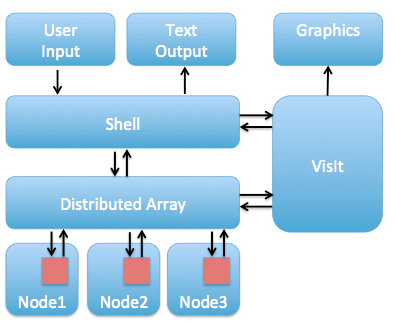
\includegraphics[width=0.53\textwidth]{communication.jpg}
	\end{center}
	\caption{Communication diagram illustrating user interaction with the shell
	controlling operations involving the distributed array and VisIt graphics.}
	\label{fig:communication}
	\vspace{-10pt}
\end{wrapfigure}

Having developed a distributed array which is accessible from both low and high-level 
languages we can address the processing of large data sets.  In particular, we seek 
ease the burden of post-processing the output of large simulations. 
The first component of this is that the distributed array must have an interface that 
automatically manages the details of the array distribution and communication.  
Additionally, we will provide an interactive shell that has variable name completion, 
history, and other user's-time saving features.  For such a shell, this project will 
rely heavily the IPython project, whose backend kernel was recently rewritten to be a 
sophisticated many-to-many parallel compute architecture.  Finally, this data analysis 
platform must be capable of visualization.  Here, we will integrate with LLNL's own VisIt 
project.  VisIt is used across many domains for dynamic, distributed, 
high-performance visualization.

%___________________________________________________________________________

\section*{Significance and Potential Impact}

Because high-level languages lack a distributed nd-array, users must manually extract a subset
 of ``interesting'' data from a larger dataset that will fit in memory on a single node.  This extraction process typically manifests 
as a serial script that slowly plows through large numbers of binary files, selects the 
important data out, and copies it to a second, smaller file.  The final decimated data fits 
in memory and the scientist may then use familiar tools.   However this decimation often takes 
hours (or days) and must be repeated if the initial selection does not contain the desired 
information.  Such repeated decimation is a gross waste of time and materials when considering 
the large number of scientists who currently employ this data management design pattern and
the lack of new fundamental knowledge gained from the practice.

The significance of this proposal, therefore, is that it would remove much of the friction 
associated with working with large datasets.  Though the individual components of the 
proposal - distributed arrays, interactive interpreters, and parallel visualization - are 
not novel concepts, coherently integrating them is.  This proposal represents a large 
advance in the capabilities available to all scientists who must work with large data, 
independent of their individual computational abilities.

There are three main thrusts of this proposal: a Python-wrapped distributed array, integration 
of this distributed array with parallel compute architecture of IPython, and fully exposing 
the distributed array data to VisIt.  

The NumPy n-dimensional array is the bedrock on which the Python scientific computing stands.  
It provides a powerful and flexible high level (Python) interface, as well as a C-API that 
allows it to easily interface with pre-existing code bases (LAPACK, etc).  The distributed 
array aims to be for parallel datasets what the NumPy \texttt{ndarray} is for serial datasets.

Moreover, augmenting the already powerful VisIt with a mechanism to directly manipulate the 
data would represent a large jump in visualization capability.  VisIt users would be able 
to invent quantities to visualize without the intermediate step of putting it in a binary 
file or relying on VisIt to anticipate a particular transformation.

% TODO
It is important that 
scientists have the tools to easily and efficiently understand the output of their
simulations.  While we are developing these technologies in the context of post-processing HYDRA output, 
they will apply to most problems where a distributed array is the correct abstraction.  
For example, this platform would be very easily adapted for use with the laboratory's large 
design codes.

% imagination, genomic datasets, lazy evaluation, fancy high level linear algebra

% TODO management
% TODO external sponsors
% TODO dissemination

%___________________________________________________________________________

\section*{Plan of Work, Schedule and Budget}

We propose the following tasks over a two year program:

\begin{enumerate}
	\item Develop a general purpose n-dimensional array and furnish with basic data 
		re-distribution routines.  Establish performance boundaries and array distribution 
		limitations. (Terry, Grote, Scopatz, 0.75 FTE) 

	\item Python Bindings and integration within IPython (Terry, Grote 0.50 FTE)

		% TODO
	\item Integration with HYDRA's output files (Terry xx FTE)

		% TODO
	\item Extensions to VisIt expose our distributed arrays and enable parallel visualization 
		with VisIt. (Terry, Grote xx FTE)

\end{enumerate}

\begin{itemize}
	\setlength{\itemsep}{0pt}
	\setlength{\parskip}{0pt}
	\setlength{\parsep}{0pt}

	\item Funded effort = 600k
		% TODO
	\item Collaboration (unfunded) =
	\item FY2013 request =  300k
	\item FY2014 request =  300k
\end{itemize}

%___________________________________________________________________________

\section*{Desired Outcome, Leverage and Exit Strategy}

Since its founding, LLNL has been a leader in the development and application of high 
performance computational systems working on large problems.  This project would extend 
capability to working \emph{interactively} with such systems.  Studies have shown productivity 
improvements of at least a factor of two\cite{Prechelt2000} in using interpreted languages 
over compiled ones.  This project would position LLNL to reap those productivity gains even 
while simulations datasets outgrow serial processing.

The objective of the project is to develop broadly useful infrastructure for manipulating 
distributed arrays in Python.  The project will leverage LLNL's extensive experience in 
parallel computation (Grote, Koning) as well as its prominence in the parallel visualization 
community (Harrison).  Additionally, the project's external collaborators are leaders in their 
communities, Scopatz as a lead developer of the PyTables project and Oliphant as the creator of 
NumPy and SciPy.

We envision the distributed array component attracting interest from a broad community 
of potential users and contributors.  This proposal alone has interested parties 
representing two LLNL developed codes (HYDRA and Warp) and an academically developed 
astrophysics \& high-energy density physics code (FLASH).  After two years, we expect this 
project to be sufficiently mature and have sufficient outside interest to turn development 
and maintenance over to a community governance team in the model of NumPy, SciPy, and IPython.

%___________________________________________________________________________

\section*{Research Team}

\setlength{\DUtablewidth}{\linewidth}
\begin{longtable*}[c]
	{|p{0.187\DUtablewidth}|p{0.251\DUtablewidth}|p{0.260\DUtablewidth}|p{0.251\DUtablewidth}|}
	\hline
	\textbf{Team Member} & \textbf{Affiliation} & \textbf{Expertise} & \textbf{Task Area} \\
	\endfirsthead
	\hline

	Matthew Terry \newline
	0.5/0.5 FTE &
	Fusion Energy Program &
	ICF, target design, Python, HYDRA, use cases &
	PI for project direction,
	distributed array, IPython integration, HYDRA interoperability \\
	\hline

	David Grote \newline
	0.5/0.3 FTE &
	Fusion Energy Program &
	Accelerator Physics, Parallel Computing &
	MPI distributed arrays, Warp interoperability \\
	\hline

	Anthony Scopatz \newline
	0.1 FTE (FY2013 Only) &
	Flash Center, \newline
	University of Chicago &
	Pytables (Python HDF5 bindings), FLASH, Nuclear fuel cycle, HEDP &
	distributed array, HDF5 interaction, FLASH interoperability \\
	\hline

	Travis Oliphant \newline
	advising &
	Continuum Analytics &
	Python scientific computing infrastructure &
	NumPy compatibility \\
	\hline

	Cyrus Harrision \newline
	advising &
	Computation, \newline
	VisIt Developer &
	Parallel Visualization &
	Interaction with VisIt/VTK  \\
	\hline

	Joe Koning \newline
	advising &
	Engineering, \newline
	HYDRA Developer & 
	ICF, Electro-magnetics, parallel computing & 
	HYDRA interoperability \\
	\hline

	Dag Sverre Seljebotn \newline
	advising &
	Dept.\ of Astrophysics, \newline
	University of Oslo &
	Astrophysics, C-Python bindings &
	Distributed array schemes and redistribution \\
	\hline
\end{longtable*}

\newpage
%___________________________________________________________________________

\bibliographystyle{plain}
\bibliography{/users/terry10/doc/latex_files/terry}

\end{document}
